\section{时空预约闭包}
\label{sec:strc}
%% =====================================================================

本节只产出允许改写的占用集合 \(U\)：输入预约表 \(R\) 与起点占用集 \(\mathrm{Src}(\mathcal{D})\)
（定义~\ref{def:seeds}），在占用之间建依赖图并取传递闭包，输出 \(U=\mathrm{Cl}(\mathrm{Src})\)；
在 \(U\) 上如何改路属第~\ref{sec:repair}~节。

\subsection{预约依赖边}
\label{sec:closure_def}

\begin{definition}[预约依赖图]
\label{def:dep}
顶点为 \(R\) 中的走廊占用。有向边 \(r\to r'\) 表示「\(r\) 失效可能迫使 \(r'\) 改路」，包括：
\begin{enumerate}[leftmargin=1.4em,itemsep=0.15em]
\item \textbf{让行边：} 同走廊、异车、时间重叠\emph{或半开区间接壤}
(\(r.t^e=r'.t^s\))，且先进入者指向后进入者；接壤在排他语义下合法，但前者延后则后者必须让路；
\item \textbf{同车后继：} 同一车辆按时间序相邻的两条占用；
\item \textbf{同工件后继：} 同一工件工序 \(i\) 的占用指向工序 \(i+1\) 的占用；
\item \textbf{同机后继：} 同一机器时间轴上相邻两道工序所诱导的占用之间的边。
\end{enumerate}
由此得到 \(G_R=(R,E_R)\)。
四类边的示意见图~\ref{fig:graphs}(b)。同工件后继连的是相邻工序所诱导的占用，
同机后继连的是同一机器时间轴上相邻两道工序所诱导的占用；
二者都以段为端点，与第~\ref{sec:shop}~节的粒度一致。
四类边只回答一个问题：\(r\) 改写之后 \(r'\) 是否可能必须跟着改。
边集是建模选择，其完备性由第~\ref{sec:e3}~节的差分试探检验。
\end{definition}

\begin{definition}[\STRC{}]
\label{def:strc}
对起点占用集 \(S\subseteq R\)、视界 \(H\) 与时刻 \(t_{\mathrm{now}}\)，
记决策时刻尚未结束、且开始时刻早于视界的占用为
\[
R^{\circ}=\bigl\{\,r\in R:\ r.t^e>t_{\mathrm{now}},\ r.t^s<H\,\bigr\},
\]
并令 \(G_R^\circ\) 为 \(G_R\) 在 \(R^{\circ}\) 上的诱导子图。
时空预约闭包的结果集合，即预约影响集，定义为
\[
\mathrm{Cl}(S)
=\bigl\{\,v\in R^{\circ}:\
\exists\,s\in S\cap R^{\circ}\ \text{使}\ s\!\to^*\!v\ \text{于}\ G_R^\circ\,\bigr\},
\]
即从尚未结束的起点占用出发，沿出边可达的全部尚未结束的占用（含起点自身）。
本文全部实验取 \(H=C_{\max}(\mathcal{S}^0)+1\)，此时 \(r.t^s<H\) 对 \(\mathcal{S}^0\) 中每条占用
都成立、视界不起筛选作用，保留 \(H\) 只为使定义可用于滚动视界。
若以邻接表表示 \(G_R^\circ\)（记其边集为 \(E_R^{\circ}\)），则可用队列在
\(O(|R^{\circ}|+|E_R^{\circ}|)\) 时间内算出；该界未单独计时，
划界只是第~\ref{sec:cheap}~节毫秒量级结果的一个组成部分。
\end{definition}

图~\ref{fig:closure} 给出示意：(a) 阻断窗与作为起点的占用；(b) 依赖边与预约影响集的边界：
集外占用不是集内占用的出边后继（命题~\ref{prop:struct}）。

\begin{figure}[t]
\centering
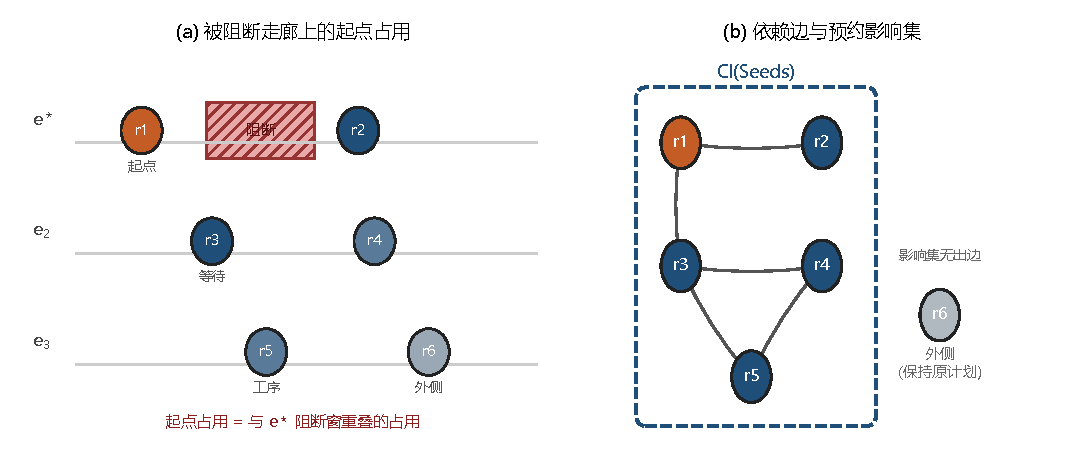
\includegraphics[width=\linewidth]{figures/fig_strc_closure_CN}
\caption{预约影响集的构造示意。
(a)~与走廊阻断窗重叠的占用作为起点；
(b)~沿四类依赖边（让行，以及同车、同工件、同机三类接续）取传递闭包得到
\(\mathrm{Cl}(\mathrm{Src})\)，集外占用保持原计划。}
\Description{两小幅示意图。(a) 时空图上一段阻断窗覆盖若干条占用，
这些占用被标为起点。(b) 从起点沿有向依赖边做传递闭包，得到预约影响集的边界；
边界之外的占用没有来自集内的入边，保持原计划。}
\label{fig:closure}
\end{figure}

按工序依赖图划界的对照，把 \(T_{\mathrm{impact}}\) 映射为允许改写的占用：
凡任务标签属于该影响域且 \(t^e>t_{\mathrm{now}}\) 的占用。
由命题~\ref{prop:miss},B 类上该集合为空。
按预约影响集划界时取 \(U=\mathrm{Cl}(\mathrm{Src})\)。
实验表中二者分别记为 R1 与 R2。

\subsection{包含性}
\label{sec:containment}

\begin{prop}[结构闭合性]
\label{prop:struct}
对任意 \(S\subseteq R\)，在 \(G_R^\circ\) 中不存在边
\(u\to v\) 满足 \(u\in\mathrm{Cl}(S)\) 且 \(v\in R^{\circ}\setminus\mathrm{Cl}(S)\)。
因而，从 \(\mathrm{Cl}(S)\) 出发沿出边无法到达影响集外、尚未结束的占用。
\end{prop}

\begin{proof}
若存在这样的边 \(u\to v\)，则由 \(u\in\mathrm{Cl}(S)\) 知存在尚未结束的起点占用 \(s\) 使
\(s\to^* u\)。拼接 \(u\to v\) 得 \(s\to^* v\)，故按定义~\ref{def:strc} 应有
\(v\in\mathrm{Cl}(S)\)，矛盾。
\end{proof}

命题~\ref{prop:struct} 说明「局部」对应一个图论上闭合的对象：影响集外的占用不是任何
集内占用的直接后继。边集固定后，闭合性即为定义的推论；其物理完备性取决于边集的选取。

\begin{remark}[预约影响集与最小允许改写集合]
\label{rem:minimality}
结构闭合性只说明影响集对所建模的依赖边封闭：集内占用没有指向集外的依赖边。
它既不保证影响集足以恢复可行，也不说明影响集不过大。后者的理由有三。

其一，\textbf{最小允许改写集合依赖于所用的修复程序，而预约影响集不依赖}。
称集合 \(U\) 为最小，须指明「在何种修复能力下 \(U\) 足以恢复可行」。允许改派与改序时的最小 \(U\)，
与只允许改路时的最小 \(U\) 不是同一个集合。预约影响集由 \(G_R\) 唯一确定，与修复程序无关——
因而它在定义上不绑定于某一启发式，也不可能同时是依赖修复程序的最小集。

其二，\textbf{四类边会多纳入不必改写的占用，而已知会漏纳的接壤情形已并入让行边}。
让行边按「同走廊、异车、重叠或接壤」建立，只要重叠即连边，而不判断后者是否\emph{真的}
只能靠等待前者通过——若该处另有旁路，后者改道即可，本不必纳入允许改写的集合；同车后继边同样
可能把延误无法传到的链尾一并纳入。这两处使影响集偏大。
反方向上，半开区间首尾相接（接壤）在排他语义下合法，但前者延后则后者必须让路，
故接壤也按让行边连接；差分试探在 \(\NPairs\) 对上的泄漏为 \ProbeLeaks（\ProbeLeakPairs；
第~\ref{sec:limitations}~节）。这一检验针对的是已知的接壤漏边，并不证明边集完备。

其三，\textbf{实测上影响集并不小}。第~\ref{sec:e6}~节报告，走廊阻断下预约影响集平均覆盖
\(t_{\mathrm{now}}\) 之后尚未结束占用的约 \ClosureAliveFrac；即相对「把决策时刻尚未结束的占用全部纳入改写」这一平凡
上界，影响集少纳入的不足一成。有界修复的节省主要来自\emph{不改写已经结束的占用}与\emph{不重新启动搜索}，
而不是大幅缩小待改写的未来占用；「局部」「有界」不意味着改动范围很小。

「不足一成」是允许改写集合的\emph{规模}之比，不等于改动比例之差。
第~\ref{sec:cheap}~节把上述平凡上界作为一条独立对照(RA)实测后发现，正是这不足一成的
差别，把改动比例从 \ResFracAllFuture\ 降到 \ResFracCheapRtwo（逐格 \RAStabWTL,
\(p=\RAStabP\)），而算法耗时与完工时间几乎不变。

因此，本文给出的是由结构唯一确定、可复现、对依赖边封闭的允许改写集合，
且在本文全部实验中均足以恢复可行；逼近最小允许改写集合是另一个问题，列为后续工作
（第~\ref{sec:future}~节）。
\end{remark}

\begin{prop}[外侧字段不变的充分条件]
\label{prop:outside}
设允许改写的占用集合 \(U=\mathrm{Cl}(S)\)，并设第 1 级改路按第~\ref{sec:level1}~节执行：
(i)~禁行窗已写入路由层；(ii)~对每个 \(r\in R^{\circ}\setminus U\)，将其原字段
\((e,[t^s,t^e),k)\) 预提交到新预约表且预提交成功；
(iii)~仅对 \(U\) 内运输调用路由器生成新占用；(iv)~最终排程通过无冲突校验。
则在恢复后的预约表 \(R'\) 中，每条 \(r\in R^{\circ}\setminus U\) 的走廊、时段与车辆与
\(\mathcal{S}^0\) 一致。此处量词是逐\emph{占用}而非逐任务：一道运输可能一部分占用在 \(U\) 内、
另一部分在外，那时只有集外那部分受本命题保护。
\end{prop}

\begin{proof}
由 (ii)，集外占用在重放开始前已按其原区间写入新表，且未与禁行窗冲突
（否则预提交失败）。步骤 (iii) 只为 \(U\) 内任务提交新占用，不删除或改写已提交的
集外区间。因此，对集外任务标签，新表中的 \((e,[t^s,t^e),k)\) 与预提交值相同，
亦即与 \(\mathcal{S}^0\) 相同。校验通过仅排除新占用与既有占用冲突，不改变已提交字段。
\end{proof}

前提 (i)--(iv) 是第~\ref{sec:level1}~节改路程序的执行条件，可对算法逐条核验，
与 A1--A5 那种模型级假设不同类，故不并入编号假设体系；命题此外依赖
A1（初始排程可行，否则集外原字段之间就可能互相冲突、预提交必然失败）、
A2（已结束占用不回溯）与 A4（走廊排他）。

\begin{remark}[前提 (ii) 与 (iii) 各自会怎样失效]
\label{rem:precommit}
若预提交因「集外占用与禁行窗重叠」失败，则 \(S\) 未能覆盖全部与阻断窗重叠的占用，起点集不完备。
若改路因运输--工序衔接失败而触发第~\ref{sec:scope_escalation}~节扩大范围，则新的允许改写集合
\(U'\supsetneq U\)，命题~\ref{prop:outside} 只对最终未纳入改写的集外占用成立。
扩大范围以可行性优先于改写尽可能少，实验中单独报告。
还有一种失效不在命题的可控范围内，但在实现上容易发生：前提 (iii) 要求路由器\emph{只}
为 \(U\) 内的运输生成新占用。若实现以比占用更粗的单位（例如整道运输、整个工序）决定
是否改路，则 \(U\) 外的占用会被一并改写，前提 (iii) 不再满足，命题的结论随之不成立。
注~\ref{rem:e2b_history} 记录了实现中出现过的这一情形及其修正。
\end{remark}

\subsection{结构可预测性}
\label{sec:structure}

预约影响集的规模由 \(G_R\) 唯一确定，排程与路网给定后没有可调参数。第~\ref{sec:instscale}~节把算例从 \(8\times4\times4\) 放大到
\(\ScaleJobsHi\times\ScaleMachHi\times\ScaleMachHi\)，影响集占比在
\ScaleCloLo--\ScaleCloHi\ 间波动，未随规模增大而上升（该比以全表为分母，其可达上界约为
\ScaleAliveShare；以可改写集合为分母时为 \ScaleCloAliveLo--\ScaleCloAliveHi）。
因而「局部」的范围可以测量，但其规模并不小（注~\ref{rem:minimality}）。

至于\emph{哪种}结构对应更大的影响集，实验结果是否定性的。
本文考察一类只由路网算出、不随当前排程变化的指标：把装卸站与车间其余部分隔开所需切断的最少走廊数，
即装卸站最小割（下称 LU 割），以及漏斗占比；下文把这一族指标称作静态割。
\textbf{影响集规模不由静态割决定}。在自建的同规模布局上，不同边界阻断协议下的
相对规模或落在很窄的带内、或虽有方向但各随机种子上的取值高度重叠；换用一批不由本文设计的路网后，
LU 割与漏斗占比\emph{取值恒定}，而影响集占比在同一张路网上换用三种机器配置
（\(6\)、\(7\)、\(8\) 机）时即明显变化；取值恒定的指标无法解释一个变化的量
（第~\ref{sec:e4}~节）。
这一否定只针对静态割；由于可得的公开路网有限，路网结构与影响集规模的一般关系尚无法判断。
下一个候选刻画应是随排程而变的量，而非纯拓扑量（第~\ref{sec:future}~节）。

%% =====================================================================
\section{预约影响集上的有界修复}
\label{sec:repair}
%% =====================================================================

图~\ref{fig:framework} 总览本节流程：先按预约影响集划定允许改写的占用集合 \(U\)，
再只对集内运输改路、集外保持原计划；仍不可行则扩大 \(U\) 再试。
按工序依赖图划界的对照只替换 \(U\) 的来源；全局重调度对照则在限定时间内重新搜索。
各方法共用同一套走廊路网、时间窗路由与无冲突校验。

\begin{figure}[t]
\centering
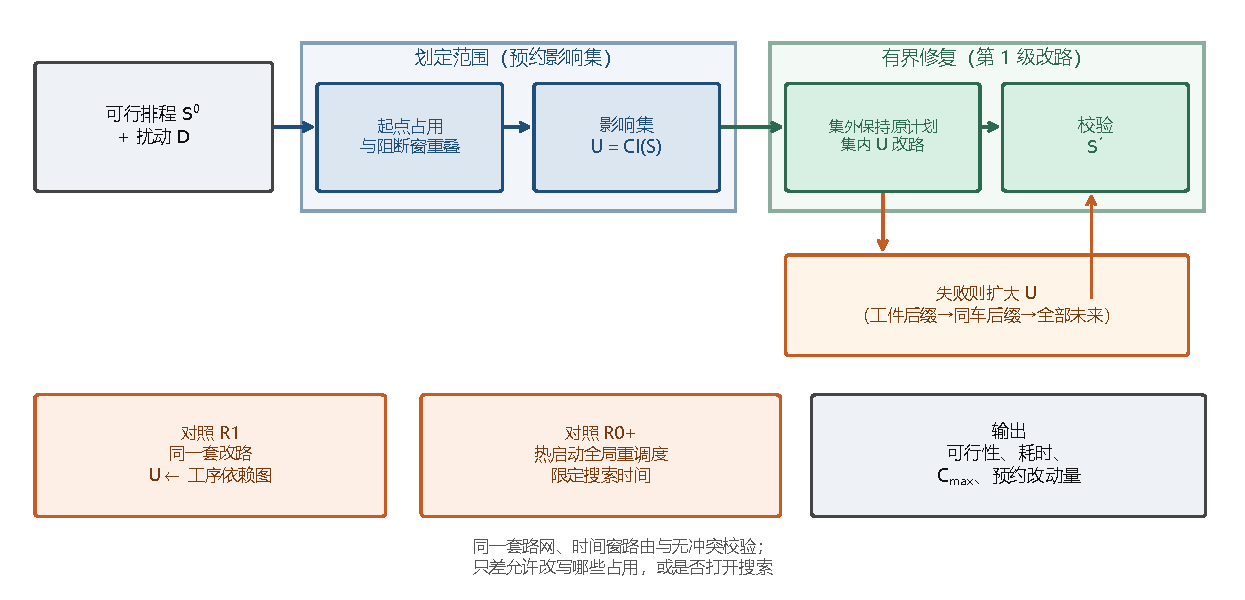
\includegraphics[width=\linewidth]{figures/fig_strc_framework_CN}
\caption{按预约影响集划界的有界修复。
上排：由起点占用得到影响集并改路；中排：失败后扩大允许改写的范围；
下排：按工序依赖图划界的对照与热启动全局重调度对照，以及输出指标。
本图只画方法层的三条路径；毫秒量级内另有三条对照（第~\ref{sec:cheap}~节）。}
\Description{三排流程图。上排：扰动进入后由起点占用得到预约影响集，集内占用允许改写、
集外保持原计划，然后原车辆改路。中排：改路失败时按工件后缀、同车后缀、
全部尚未结束占用的顺序扩大允许改写的集合并重试。下排：两条对照，
一按工序依赖图上的影响域划定范围，一做热启动全局搜索；三条路径汇入同一组输出指标。}
\label{fig:framework}
\end{figure}

\subsection{允许改写、保持原计划与第 1 级改路}
\label{sec:level1}

给定允许改写的占用集合 \(U\)，第 1 级改路保持原车辆指派与机器指派，按原加工顺序重放。
改路以走廊路段（即一次行驶中通过单条走廊的一段，下称路段）为粒度：车辆在 \(t_{\mathrm{now}}\)
前已通过的路段属于已完成占用，原样预提交，改路只从车辆当时所在的节点开始规划；
若粒度粗于路段，就会改写已完成的占用（注~\ref{rem:e2b_history}）。
算法~\ref{alg:replay} 给出这一原语；算法~\ref{alg:strc_repair} 在其外层计算预约影响集，失败时扩大 \(U\)。

\begin{algorithm}[t]
\caption{第 1 级改路重放 \(\textsc{ReplayReroute}\)}
\label{alg:replay}
\begin{algorithmic}[1]
\Require 排程 \(\mathcal{S}^0=(x,\pi,y,R)\)，扰动 \(\mathcal{D}\)，允许改写集合 \(U\)，时刻 \(t_{\mathrm{now}}\)
\Ensure 排程 \(\mathcal{S}'\) 或失败
\State 将 \(\mathcal{D}\) 写入路由层
  \Comment{阻断：禁行窗；通行变慢：重叠段 \(\tau\)}
\State 取空表 \(R'\)
\For{每条不可改写的占用：集外的全部，以及 \(r\in U\) 而 \(r.t^e\le t_{\mathrm{now}}\) 的}
  \State 将原字段 \((e,[t^s,t^e),k)\) 预提交到 \(R'\)
    \Comment{第二类是 A2 规定的已完成占用，遗漏即等于改写它们}
  \If{与阻断窗冲突}
    \State \Return 失败
      \Comment{起点占用未覆盖与窗重叠的占用}
  \EndIf
\EndFor
\For{每条 \(r\in U\)，按原加工顺序}
  \State 从该车辆在 \(t_{\mathrm{now}}\) 所在的节点开始规划 \Comment{已通过的路段已在上一步预提交，不重复提交}
  \State 在当前 \(R'\) 上调用时间窗路由，提交新占用
    \Comment{不改写已经结束的占用}
\EndFor
\State 按 \(\pi\) 推进各机器空闲时刻与各工件就绪时刻
\State 独立校验：无冲突、无禁行窗残留、通行变慢的重叠段时长已吸收、集外字段未改
\If{校验通过}
  \State \Return \(\mathcal{S}'=(x,\pi,y,R')\)
\Else
  \State \Return 失败
\EndIf
\end{algorithmic}
\end{algorithm}

划界那一遍广度优先（定义~\ref{def:strc}）只占耗时的一小部分：一次
\(\textsc{ReplayReroute}\) 还要对 \(|U|\) 个运输段各调用一次时间窗最短路，
实测耗时由后者主导（第~\ref{sec:e3}、\ref{sec:cheap}~节）。
该级不启动种群搜索。第~\ref{sec:e3}~节的对照固定算法~\ref{alg:replay}，只替换 \(U\) 的来源（工序依赖图或预约影响集），
用以把可行率之差归因于划界对象。

\subsection{失败后扩大允许改写的范围}
\label{sec:scope_escalation}

扩大允许改写的范围，本身已有成例。Local Rescheduling~\cite{kuster2007local}
按时间窗逐步放宽直至可行；AOR 则按工件后继与同机后继纳入后续工序
（第~\ref{sec:rw_aor}~节）。本文沿预约依赖边扩大 \(U\)，而不是沿时间窗。
这些步骤用于落实影响集：改路失败时先扩大须改写的占用，而不是立即转为全局搜索。
第~\ref{sec:protocol}~节说明边界消融实验为何必须关闭这一步。

当集外占用保持过紧时，算法~\ref{alg:replay} 可能因运输--工序衔接等校验失败。
此时按下列顺序扩大 \(U\) 并重试同一套改路程序：
(i)~\(U\leftarrow U\cup\{\)当前 \(U\) 内各工序的同工件后缀、尚未结束的占用\(\}\);
(ii)~\(U\leftarrow U\cup\{\)所涉车辆的同车后缀、尚未结束的占用\(\}\);
(iii)~\(U\leftarrow\{\,r\in R:\ r.t^e>t_{\mathrm{now}}\,\}\)（把决策时刻尚未结束的占用全部纳入改写）。
扩大范围后仍是确定性的单遍改路。实验中这一步使全部格恢复可行，算法耗时保持在毫秒至十余
毫秒量级（第~\ref{sec:experiments}~节）。耗时随扰动比例 \(\varphi\) 并非单调变化，
一种可能的解释是两种效应方向相反：比例小时初始影响集偏紧、更常需要扩大范围；比例大时初始 \(U\) 已较宽、
往往一轮即成功，但单轮需要改路的运输更多（结果见第~\ref{sec:scale}~节）。

\subsection{与全局重调度的对照}
\label{sec:vs_r0}

全局重调度对照在相同禁行约束下、在限定时间内以原排程为起点重新搜索（记 R0+）。
内部把 \((x,\pi)\) 编成一条染色体；一次\emph{解码}指：按该染色体的指派与加工顺序，
在已写入禁行窗的预约表上从头为全部运输调用第~\ref{sec:reservation}~节的时间窗路由，
得到新的 \(R\) 与 \(C_{\max}\)。R0+ 重复解码并允许改染色体；第~\ref{sec:cheap}~节的
RD 只解码一次且不改染色体。R0+ 的解码不改写已经结束的占用：这些占用预提交，
只从 \(t_{\mathrm{now}}\) 起排定尚未开始的工序（第~\ref{sec:e5}~节）。
对照取热启动而非从零搜索，以免丢掉原排程已有的指派与路径信息。
R0+ 可改派与改序，因而更可能缩短 \(C_{\max}\)，但算法耗时由预算决定。

有界修复在完工时间上并不优于 R0+。第~\ref{sec:e5}~节表明：R0+ 在最小预算档上已占优，
而 R2 的结果不随预算变化、R0+ 的 \(C_{\max}\) 随预算单调不增，故增加预算也不出现反超。
有界修复的长处在于算法耗时：响应须在毫秒量级时，它能恢复可行；允许秒级停机时，应采用 R0+ 缩短 \(C_{\max}\)。
集外占用的走廊、时段与车辆保持原计划，由命题~\ref{prop:outside} 在其条件下保证。

仅与 R0+ 对照留下一个问题：在毫秒量级的耗时内，按影响集划界是否必要?
为此本文实现三种不按影响集限制范围的做法：全局右移(RS)不判断哪些占用
受影响，只把未完成占用整体后推到阻断结束之后；原染色体重解码(RD)不改染色体，只执行一次固定前缀解码；
\textbf{RA} 把 \(t_{\mathrm{now}}\) 之后尚未结束的占用全部纳入改写，再执行与第~\ref{sec:level1}~节
\emph{完全相同}的改路程序，因而与本文方法只差「允许改写哪些占用」这一项，是唯一能单独检验预约影响集
作用的对照。三者耗时均在毫秒量级，构成有界修复在\emph{同一耗时量级内}的对照，
定义与结果见第~\ref{sec:cheap}~节。

算法~\ref{alg:strc_repair} 把本节与上节合起来写出，与图~\ref{fig:framework} 对应。

\begin{algorithm}[t]
\caption{基于预约影响集的有界修复（第 1 级改路 + 扩大范围）}
\label{alg:strc_repair}
\begin{algorithmic}[1]
\Require 排程 \(\mathcal{S}^0\)，扰动 \(\mathcal{D}\)，时刻 \(t_{\mathrm{now}}\)
\Ensure 排程 \(\mathcal{S}'\) 或失败
\State \(S \gets \mathrm{Src}(\mathcal{D})\);
      \(U \gets \mathrm{Cl}(S)\)
\For{轮次 \(=0,1,2,3\)}
  \State \(\mathcal{S}' \gets \textsc{ReplayReroute}(\mathcal{S}^0,\mathcal{D},U,t_{\mathrm{now}})\)
  \If{\(\mathcal{S}'\) 可行}
    \State \Return \(\mathcal{S}'\)
  \EndIf
  \State 按扩大范围的规则更新 \(U\) \Comment{工件后缀 / 同车 / 全部尚未结束}
\EndFor
\State \Return 失败
\end{algorithmic}
\end{algorithm}

%% =====================================================================
